% !TEX root = SegwayDoku.tex
\newpage
\renewcommand{\autoren}{Valentyn Chepil}
\section{Das Gehäuse}
\subsection{Das Gehäuse - V.1}
% \ref{bild_3} zuweisung auf Bild in Text.
\begin{figure}[!h]  % [h] bedeutet, dass das Bild genau an dieser Stelle im Text erscheint
	% mit width=... wird die Größe des Bildes in Prozent der Seitenbreite eingestellt
	\centering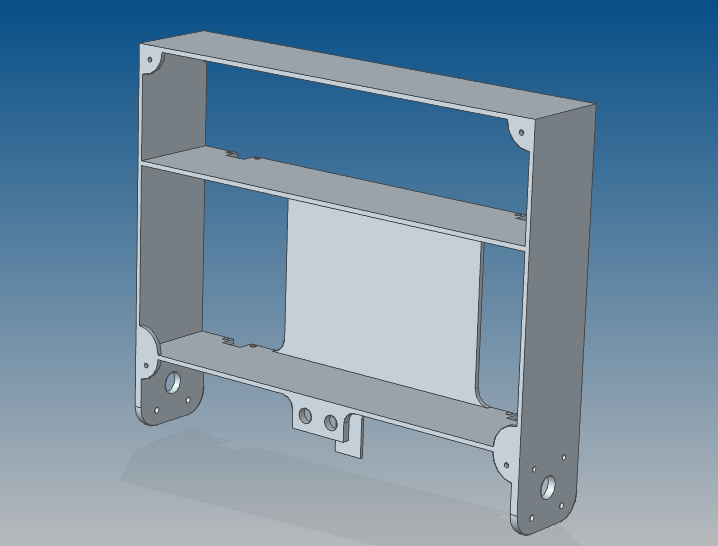
\includegraphics[width=0.5\textwidth]{images/gehaeuse-v1.png}
	% caption ist die Bildunterschrift, taucht auch im Abbildungsverzeichnis auf
	\caption{Das Gehäuse - V.1 \newline (Quelle: eigene Darstellung)}
	\label{gehaeuse-v1} % über das label kann man aus dem Text auf das Bild verweisen
\end{figure}
Es wurde gesagt, sehr einfachen Aufbau des Gehäuse im Form des Kastens herzustellen.
\subsection{Das Gehäuse - V.2}
\begin{figure}[!h]  % [h] bedeutet, dass das Bild genau an dieser Stelle im Text erscheint
	% mit width=... wird die Größe des Bildes in Prozent der Seitenbreite eingestellt
	\centering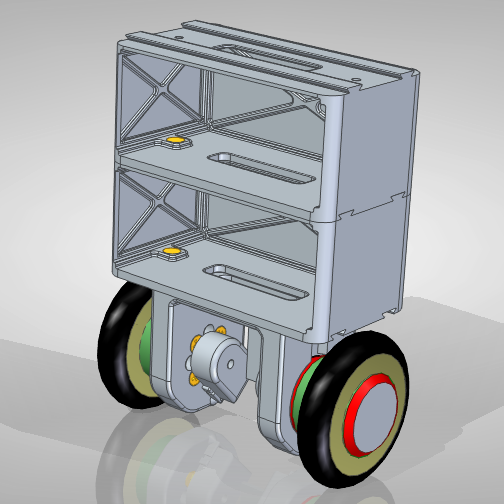
\includegraphics[width=0.5\textwidth]{images/gehaeuse-v2.png}
	% caption ist die Bildunterschrift, taucht auch im Abbildungsverzeichnis auf
	\caption{Das Gehäuse - V.2 \newline (Quelle: eigene Darstellung)}
	\label{gehaeuse-v2} % über das label kann man aus dem Text auf das Bild verweisen
\end{figure}
Im Bild \ref{gehaeuse-v2} ist eine modulare Darstellung des Roboters zu sehen. Der Motorhalter ist in diesem Fall als ein externer Modul dergestalt. Im ersten Modul von oben sollte man alle Steuerungsplatinen  einbauen. Das zweite Modul von Oben sollte  der Akku beinhalten. Mit Hilfe vom Schwalbenschwanzverbindung und zwei Schrauben sollten die Module miteinander verbindet werden.

\subsection{Das Gehäuse - V.3}

Die Version V.2 (Bild \ref{gehaeuse-v2}) unterscheidet sich nicht viel von V.3. Es wurde die modulare Aufbau nicht geändert. Da hat man Schwalbenschwanzverbindung durch Steckverbindung ersetzt, die seitlich Zugeordnet sind. Es wurde auch Motorhalter modernisiert.

\begin{figure}[!h]  % [h] bedeutet, dass das Bild genau an dieser Stelle im Text erscheint
	% mit width=... wird die Größe des Bildes in Prozent der Seitenbreite eingestellt
	\centering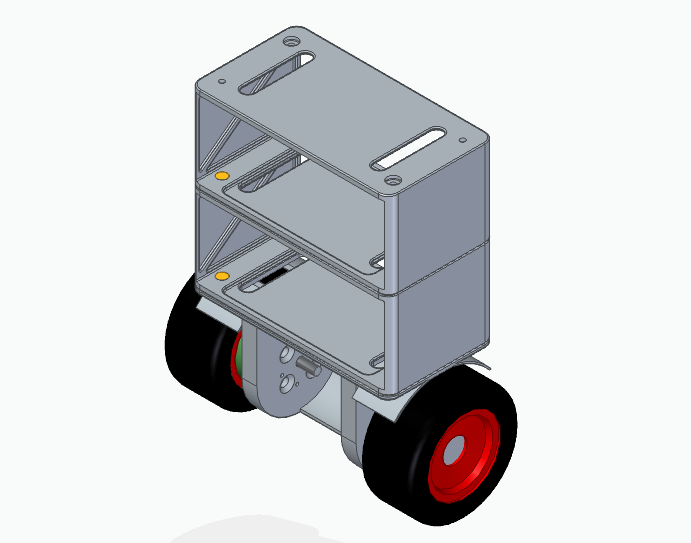
\includegraphics[width=0.5\textwidth]{images/gehaeuse-v3.png}
	% caption ist die Bildunterschrift, taucht auch im Abbildungsverzeichnis auf
	\caption{Das Gehäuse - V.2 \newline (Quelle: eigene Darstellung)}
	\label{gehaeuse-v3} % über das label kann man aus dem Text auf das Bild verweisen
\end{figure}

\subsection{Das Gehäuse - V.4}

Endgültiges Gehäuse ist auf der Abbildung \ref{gehaeuse-v4} zu betrachten. Es wurde die Version gesintert.

\begin{figure}[htb]
	\centering
	\begin{minipage}{0.45\linewidth}
		\centering
		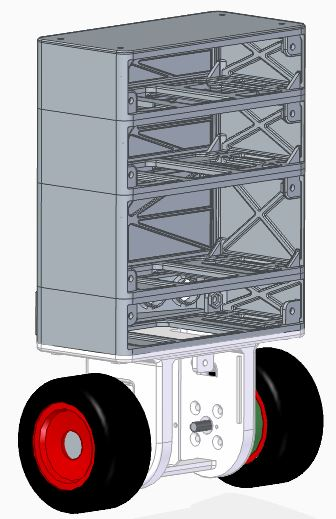
\includegraphics[scale=0.48]{images/4.1_vorne.jpg}
		\caption{Endgültiges Gehäuse V4.1 \newline(Quelle: Eigene Darstellung)}
		\label{gehaeuse-v4}
	\end{minipage}
	%\hfill
	\begin{minipage}{0.45\linewidth}
		\centering
		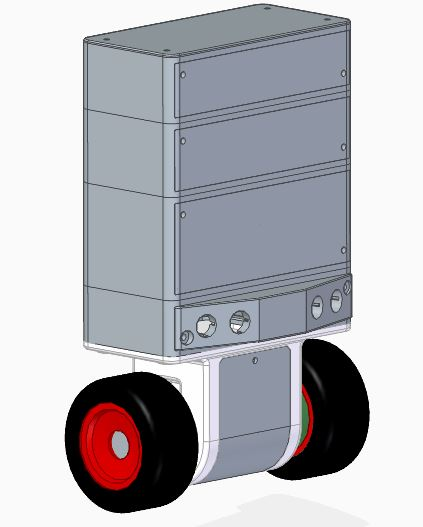
\includegraphics[scale=0.48]{images/4.1_hinten.jpg}
		\caption{ mit Deckels \newline (Quelle: Eigene Darstellung)}
	\end{minipage}
\end{figure}
\pagebreak
\subsection{Das Gehäuse - V.4.2.3}

Nach Zusammenbau des Roboters wurde folgende Korrektur noch durchgeführt:
 
\begin{itemize} 
	\item  mBed-Modul wurde 10 mm höher gemacht.
	\item  Anpassung an Kabelkanal Führung.
	\item  Beschriftung auf der Module.
	\item  Oberwand wurde komplett entfernt.
	\item  Versteifungen als Deckelsturzstelle.
	\item  Akku-Modul wurde 10 mm höher gemacht.
	\item  mBed und oDrive wurden stark nach einer Seite platziert.
\end{itemize}

\begin{figure}[htb]
	\centering
	\begin{minipage}{0.45\linewidth}
		\centering
		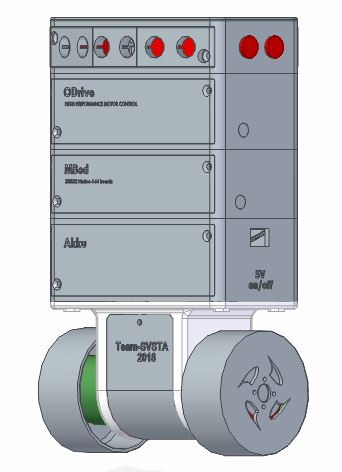
\includegraphics[scale=0.48]{images/V.4.3.jpg}
		\caption{Gehäuse V4.3 \newline(Quelle: Eigene Darstellung)}
		\label{gehaeuse-v4.3}
	\end{minipage}
	%\hfill
	\begin{minipage}{0.45\linewidth}
		\centering
		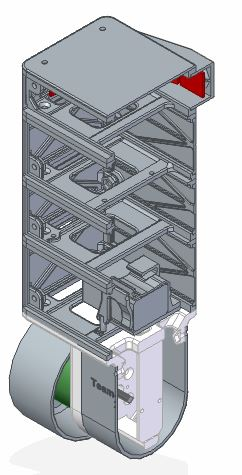
\includegraphics[scale=0.48]{images/V.4.3-1.jpg}
		\caption{ Schnitt \newline (Quelle: Eigene Darstellung)}
	\end{minipage}
\end{figure}

\subsubsection{ Berechnung vom Motorhalter}
Alle Berechnungen wurden mit Hilfe von FEM - Programmierung erstellt und beweise die Festigkeit nur von dem Motorhalter. Es wurden an den Stellen vom Motoren und Räder das Moment laut der Berechnung \ref{FEM1} verwendet und als Lastkraft von 50N wurde auf die Oberfläche eingeprägt.

Die Materialeigenschaften kann man aus der Abbildung \ref{FEM2} ablesen.
\pagebreak
\begin{figure}[!h]  % [h] bedeutet, dass das Bild genau an dieser Stelle im Text erscheint
	\centering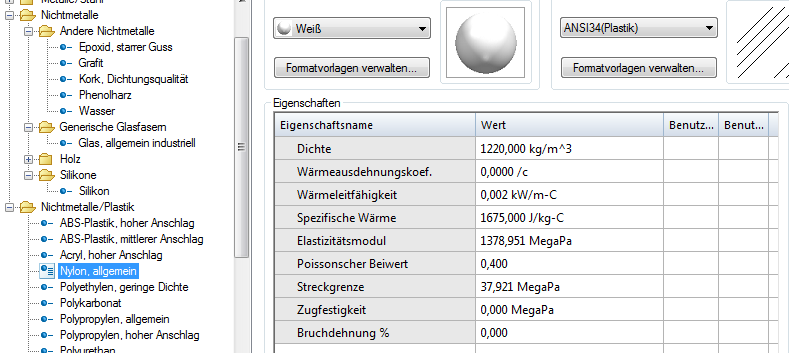
\includegraphics[width=0.7\textwidth]{images/FEM2.png}
	% caption ist die Bildunterschrift, taucht auch im Abbildungsverzeichnis auf
	\caption{Kunststoffeigenschaften - Nylon (PA) \newline (Quelle: eigene Darstellung)}
	\label{FEM2} % über das label kann man aus dem Text auf das Bild verweisen
\end{figure}

Der Motorhalter wurde minimal vernetzt, um die Berechnungszeit zu reduzieren.

\begin{figure}[!h] 
	\centering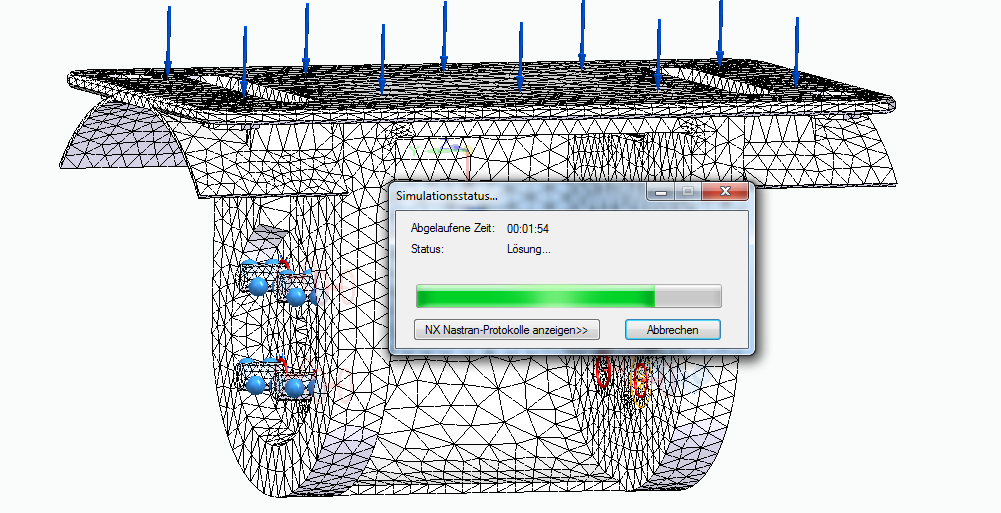
\includegraphics[width=0.8\textwidth]{images/FEM.png}
	\caption{FEM-Berechnung \newline (Quelle: eigene Darstellung)}
	\label{FEM1} % über das label kann man aus dem Text auf das Bild verweisen
\end{figure}

Es wurden die Verschiebungen und Spannungen auf das Bild \ref{FEM3} und \ref{FEM4} eingeordnet. 

\begin{figure}[htb]
	\centering
	\begin{minipage}{0.49\linewidth}
		\centering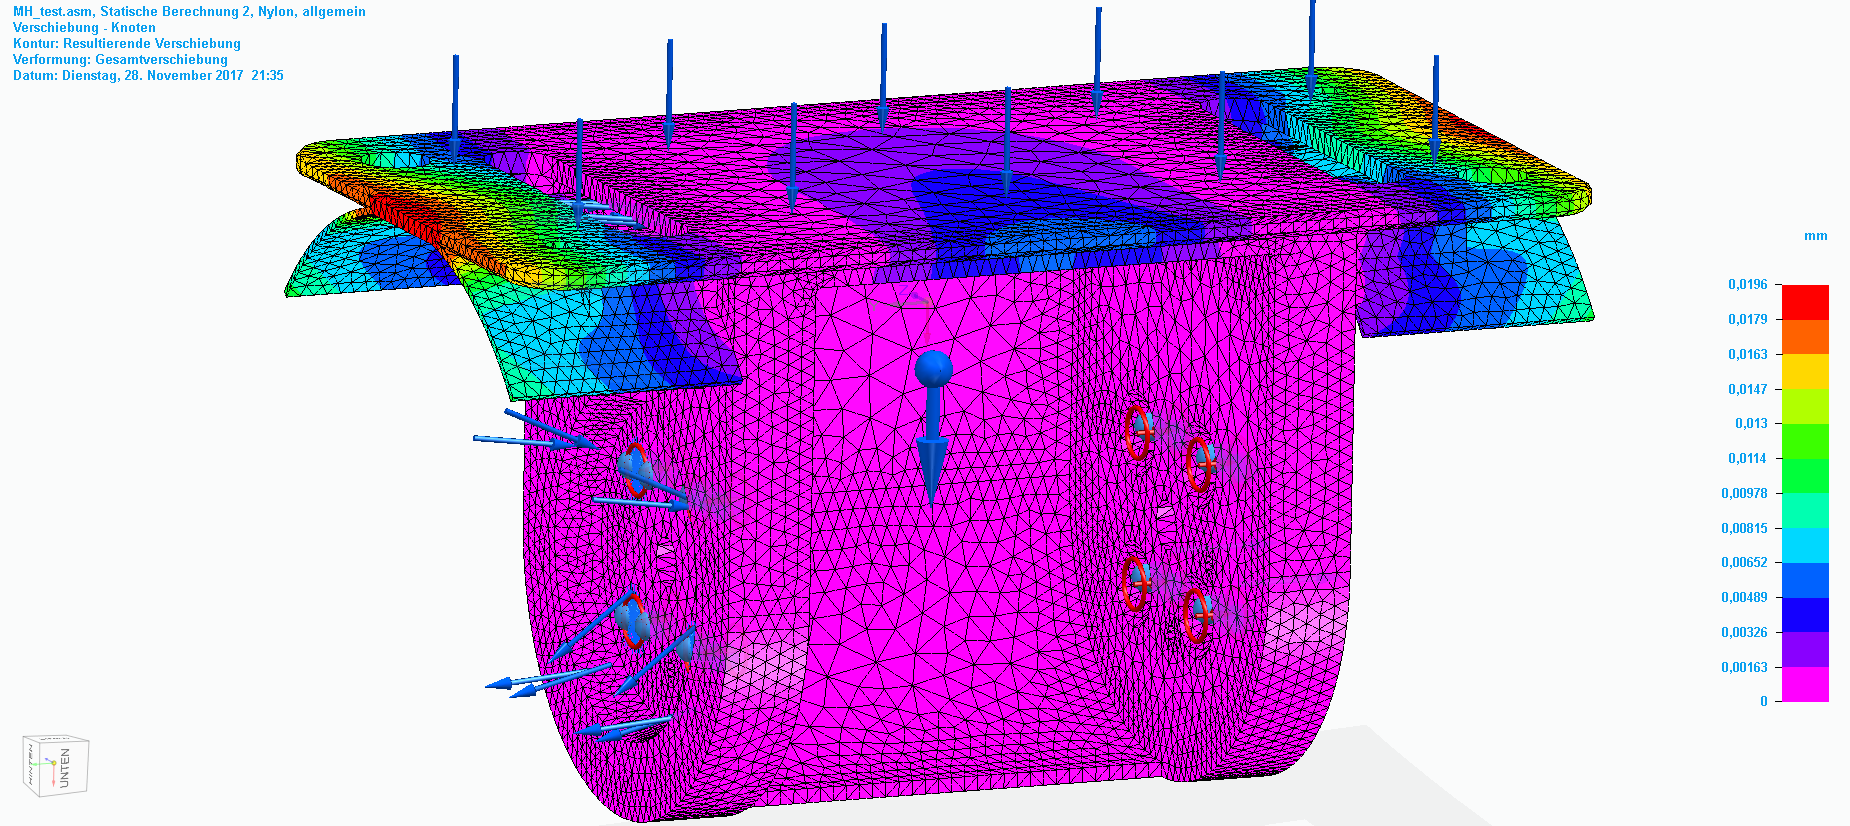
\includegraphics[width=0.9\textwidth]{images/FEM3.png}
		\caption{FEM - Verschiebungen \newline (Quelle: eigene Darstellung)}
		\label{FEM3}
	\end{minipage}
	\begin{minipage}[h]{0.49\linewidth}
		\centering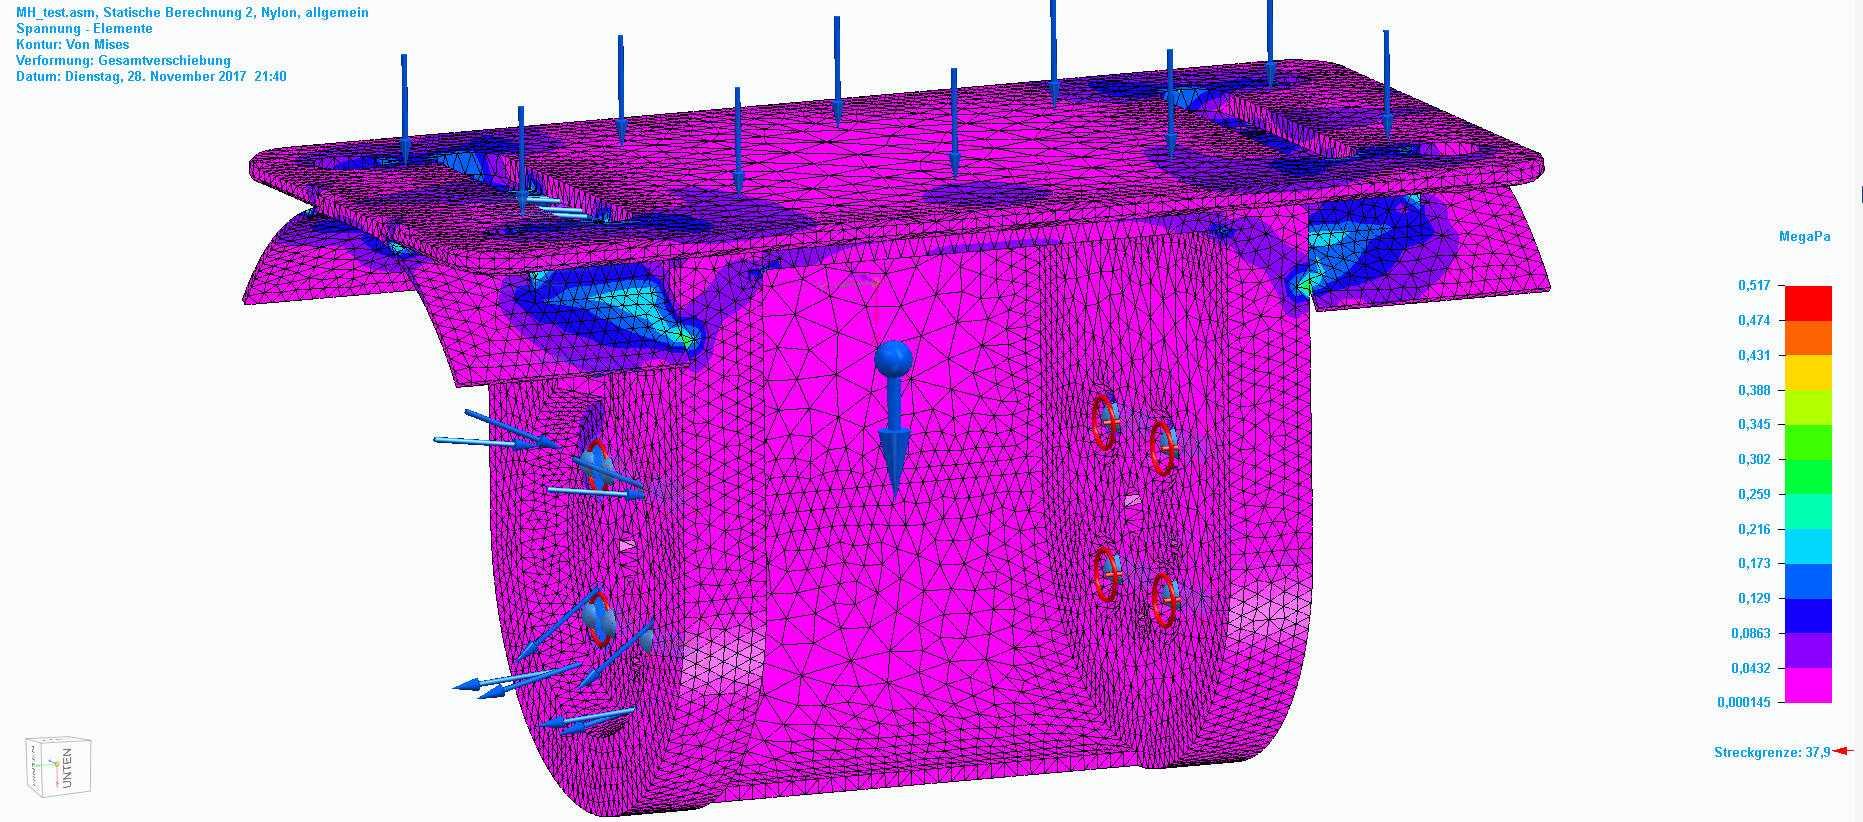
\includegraphics[width=0.9\textwidth]{images/FEM4.png}
		\caption{FEM - Spannungen \newline (Quelle: eigene Darstellung)}
		\label{FEM4}
	\end{minipage}
\end{figure}

Auf der Bilder \ref{FEM3}, \ref{FEM4} ist es zu sein, dass Sicherheitsfaktor der Festigkeit vom Motorhalter ist deutlich höher als 2 und braucht damit keine weiteren Berechnungsvorgänge.

